\documentclass[conference]{IEEEtran}
\usepackage{cite}
\usepackage{amsmath,amssymb,amsfonts}
\usepackage{algorithmic}
\usepackage{graphicx}
\usepackage{textcomp}
\usepackage{xcolor}
\usepackage{url}
\usepackage{wrapfig}
\usepackage{booktabs}  % For professional-looking tables
\usepackage{appendix}  % For appendix
\usepackage{longtable}
\usepackage{tabularx}
\usepackage{hyperref}


\def\BibTeX{{\rm B\kern-.05em{\sc i\kern-.025em b}\kern-.08em
    T\kern-.1667em\lower.7ex\hbox{E}\kern-.125emX}}
\begin{document}

\title{Traffic Flow Prediction Using LSTM Neural Networks\\
{\footnotesize \textsuperscript{}}

}

\author{\IEEEauthorblockN{1\textsuperscript{st} Ankur Jain}
\IEEEauthorblockA{\textit{VIT Bhopal University} \\
\textit
ankurjainjob.gmail.com}
\and
\IEEEauthorblockN{2\textsuperscript{nd} Arin Balyan}
\IEEEauthorblockA{\textit{VIT Bhopal University} \\
\textit
arinbalyan2022@vitbhopal.ac.in}

}

\maketitle

\begin{abstract}
Traffic flow management and prediction are important in modern transportation systems, helping commuters enhance their routes and enabling the concerned authorities to make informed decisions regarding road maintenance and development. Accurate, precise, and fast traffic flow prediction plays a crucial role in enhancing a road network's efficiency, reducing congestion, and improving the overall travel experience for commuters. 

In this research paper, we propose a method to analyze and then predict the flow of traffic using deep learning techniques and artificial neural networks, particularly through L.S.T.M. (Long Short-Term Memory) neural network. This model effectively captures both temporal and spatial dependencies found in traffic data by processing sequences of traffic indices measured at multiple sensor locations. Our approach aims to forecast future traffic conditions at 15-minute intervals, leveraging historical traffic volume data and other relevant features. The results demonstrate that our predictive model achieves high accuracy and reliability, and offers insights which helps in effective traffic management and planning.

\end{abstract}

\begin{IEEEkeywords}
Traffic Flow Prediction, Artificial Neural Networks, LSTM (Long Short-Term Memory), Deep Learning, Traffic Management Systems, Spatiotemporal Data
\end{IEEEkeywords}

\section{Introduction}
Traffic congestion is an ever-growing problem that affects people from all walks of life in their day-to-day activities, whether in a metropolitan city, a small town, or a village. Traffic jams or congestion significantly impact economic productivity and lead to substantial losses for people. It also affects the quality of life of a large populace. Precise and accurate traffic prediction is vital for enhancing and optimizing route planners and maps over the internet and reducing congestion on already congested roads. Traditional methods, such as statistical models and approaches like ARIMA (Auto-Regressive Integrated Moving Average), often struggle to comprehend the complex and dynamic nature of increased traffic flow in past few years.\\

This research explores the application of ANNs in prediction of traffic flow. The critical challenge is to model the spatiotemporal dependencies of traffic data while incorporating inputs like sensor data. Our aim from this paper is to develop a solution that can help commuters enhance their travel experience and make commuting for day-to-day activities like work and education easier for the working population and students.

\section{Applications}
The application of traffic flow prediction systems utilizing artificial intelligence encompasses a diverse range of users, including individuals, city planners, emergency responders, and logistics companies. This technology is pivotal in enhancing urban mobility and safety by providing timely and accurate traffic forecasts.
Traffic management centers benefit significantly from these predictive systems as they enable the optimization of traffic signal timings and reduction of congestion. By accurately forecasting traffic conditions, authorities can detect incidents such as accidents more swiftly, allowing for prompt responses and necessary interventions. Research has shown that machine learning algorithms can effectively enhance traffic flow predictions, leading to improved traffic management outcomes\cite{ppr25}.
Urban planners also rely on accurate traffic forecasts to make informed decisions regarding infrastructure development. By analyzing projected traffic volumes, planners can determine optimal locations for new roads or public transport facilities. Furthermore, transit authorities can adjust public transport schedules to better align with anticipated passenger demand, thereby improving service efficiency and user satisfaction\cite{ppr26}.
In emergency situations, traffic flow prediction systems are crucial for guiding emergency services to the most efficient routes, thus improving response times. These systems also play a vital role in disaster management by facilitating effective evacuation strategies based on predicted traffic conditions. Studies indicate that integrating AI-based prediction models can enhance the effectiveness of emergency response strategies.
Logistics and delivery services leverage these predictive capabilities to optimize routing and reduce travel times and fuel costs. By proactively adjusting delivery routes based on predicted traffic conditions, fleet managers can enhance operational efficiency and safety. This application is particularly relevant in today's context where timely deliveries are critical for customer satisfaction\cite{ppr26}.


\section{Background and Objectives}

The focus of this paper is to provide accurate predictions of traffic flow (potentially real-time in the future). This enables traffic management centers to make informed decisions regarding traffic signal timings and responses to incidents on roads. Emphasis is placed on leveraging large datasets, including historical traffic patterns, peak hours, holidays, and special events, to train the ANN model. This data-driven approach helps in understanding traffic dynamics. Additionally, the LSTM-based model aims to capture temporal and other time-related dependencies in the data related to traffic and recognize how traffic flow is influenced by conditions like day, date, time, and weather, which is important for predicting short-term events. Finally, importance is placed over the scalability and adaptability of the solution to ensure it is feasible for large-scale implementation. The purpose of this project is to address traffic congestion, a significant challenge in metropolitan areas that leads to increased travel time, as well as increased pollution of the environment and fuel use. Because of the oversimplified models, traditional traffic management systems often fall short in responding to the dynamic nature or essence of traffic flow. Accurate forecasting is important due to the hidden intricacies of traffic patterns, which are influenced by various variables, including the time of the day, the weather, and special events like holidays and festivals. Therefore, there is an urgent need for advanced predictive models that can leverage historical data to provide timely insights into traffic conditions.

As cities grow denser and traffic becomes increasingly complex, the need for precise traffic flow prediction has never been more critical. Urban traffic congestion poses a multifaceted challenge, directly affecting economic productivity, individual well-being, and environmental health. Despite significant advances, predicting traffic flow remains an elusive goal because of the inherently and often unpredictable essence of traffic systems. Current traffic prediction models struggle to adapt to rapid fluctuations and diverse influencing factors—ranging from peak travel times and weather variations to road accidents and special events—that drive daily traffic patterns.



\section{Dataset}

The dataset we used for this research is designed in such a way that it measured traffic volume after every 15 minutes interval and for 36 different locations for the sensor along major two highways in the capital region of Northern Virginia / Washington D.C., United States Of America. The dataset includes upto 47 features which are as follows:

\begin{enumerate}
    \item The past sequence of of traffic density for ten most sample points (10 features).
    \item Day of the week for further differentiation in analysis based on holidays and normal working days  (7 features).
    \item The specific time or hour of the day (24 features).
    \item Direction of the road (4 features).
    \item Highway's Number of lanes (1 feature).
    \item Name of the road (1 feature).
\end{enumerate}

The final task is for the prediction of traffic volume for the 15 minutes in the future for all the 36 locations sensors were installed. Given that we have a well established road network and we are aware of the spatial connectivity between the location of sensors installed. The dataset can be accessed via the following link: 
\begin{quote}
\texttt{\href{http://mason.gmu.edu/~lzhao9/pages/dataset_pages/datasets/spatial/traffic_dataset.mat}{Dataset}}\cite{dataset}
\end{quote}
\textbf{Dataset format}: .mat (Use MATLAB to access the Dataset).






\subsection{Traffic Volume Over Time}

To further understand the dynamics of traffic volumes, we analyze the traffic volume over time for Sensor 0. The plot (~\ref{fig:traffic_volume_over_time_sensor_0}) illustrates variations in traffic volume across different time intervals, revealing patterns that are critical for forecasting.

\begin{figure}[htbp]
    \centering
    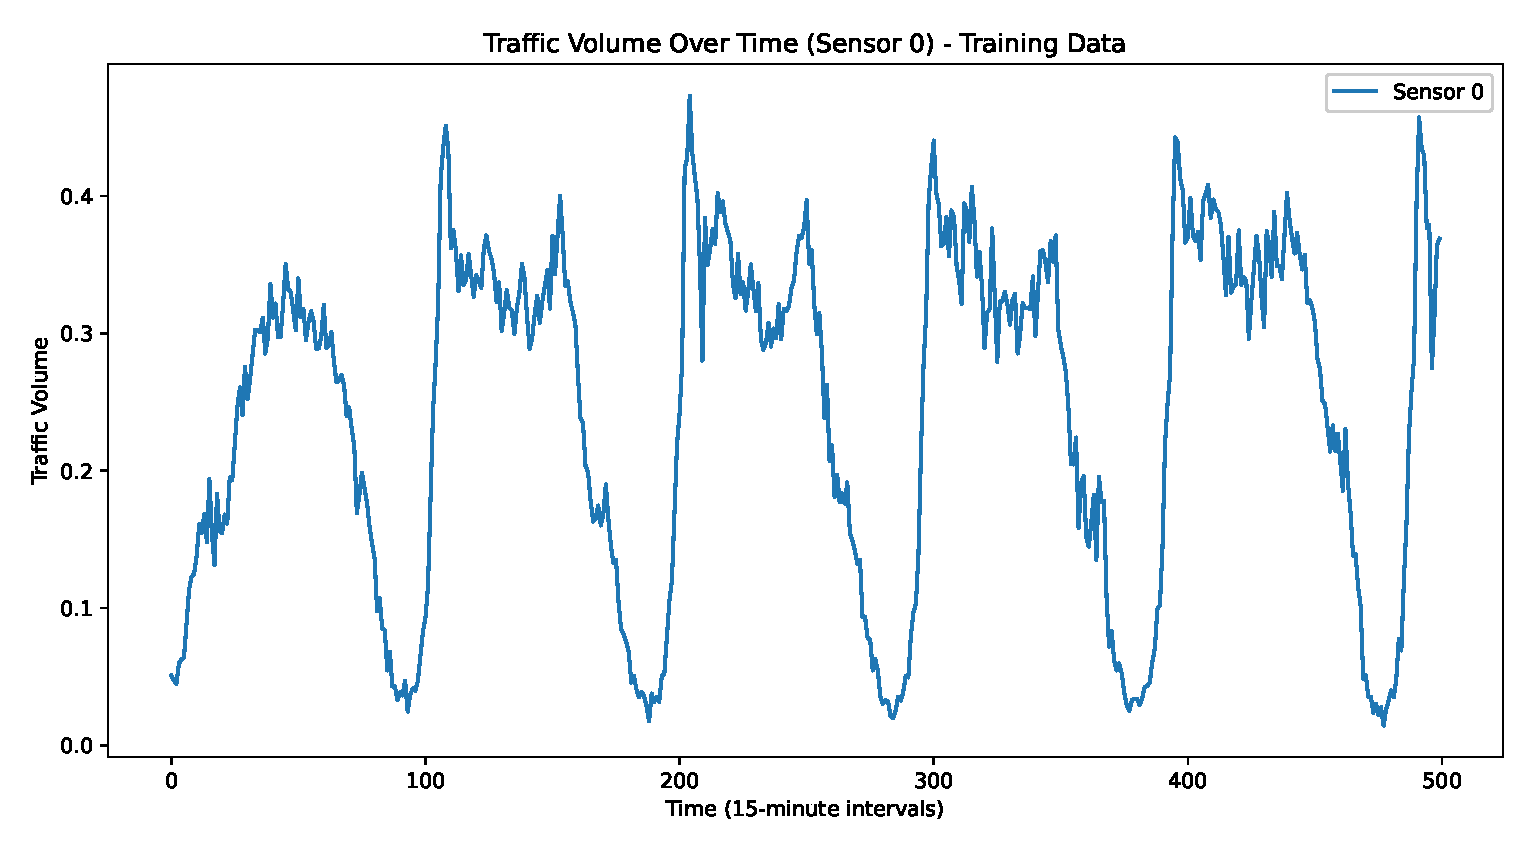
\includegraphics[width=0.5\textwidth]{images/traffic_volume.eps}
    \caption{Traffic Volume Over Time (Sensor 0) - Training Data}
    \label{figure:traffic_volume_over_time_sensor_0}
\end{figure}

The analysis of this temporal data helps identify peak traffic periods and informs the prediction model of the expected traffic flow under varying conditions.


\subsection{Average Traffic Volume by Hour}

By analyzing the average traffic volume by hour, we can determine typical traffic patterns throughout the day. This information is crucial for building accurate predictive models that account for time-of-day variations.

\begin{figure}[htbp]
    \centering
    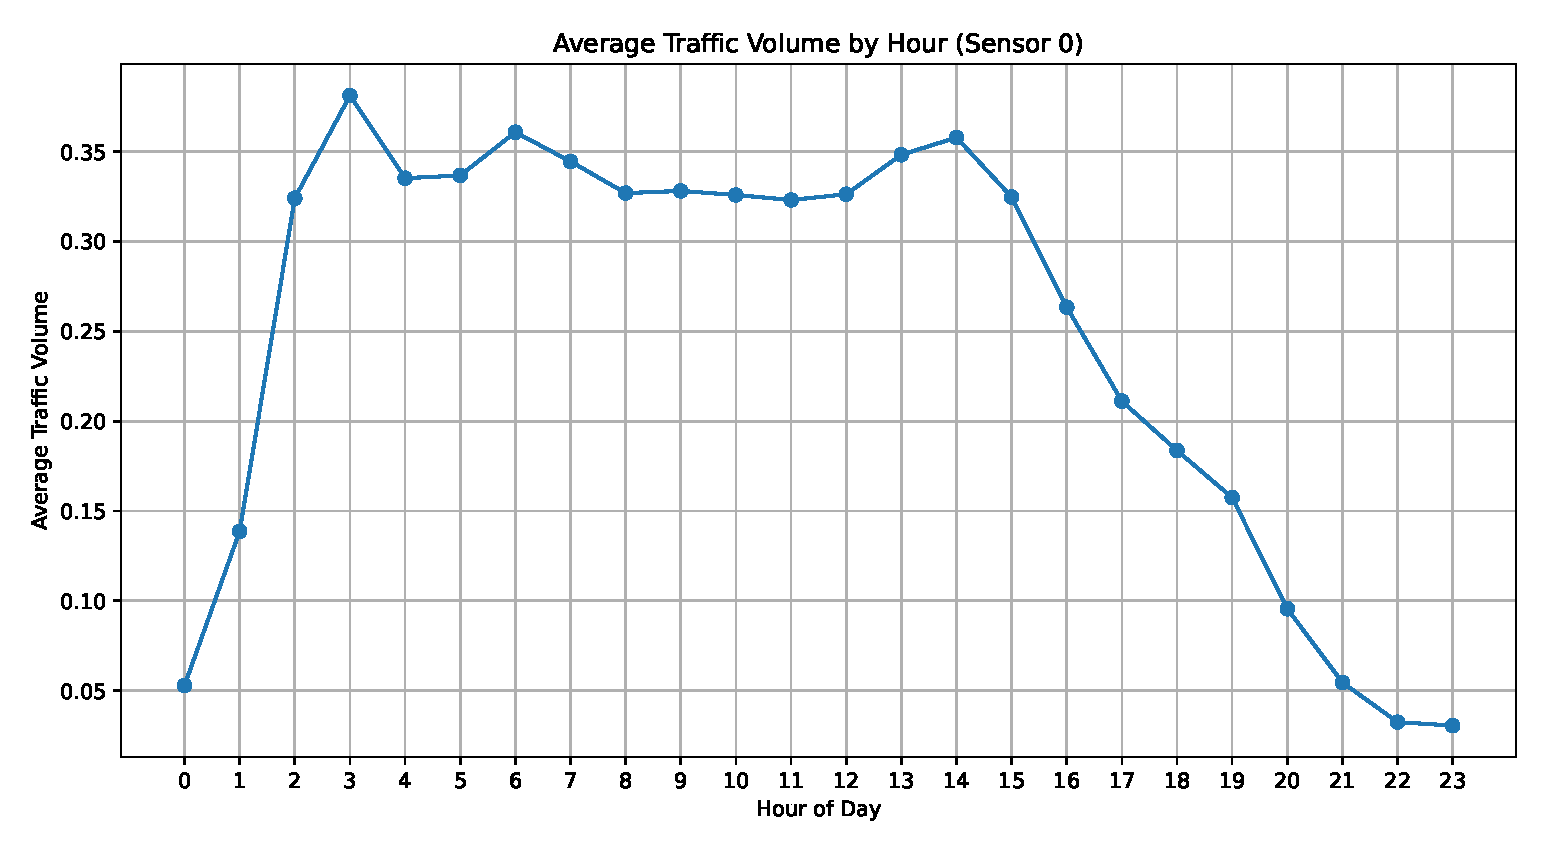
\includegraphics[width=0.5\textwidth]{images/avg_traffic_volume.eps}
    \caption{Average Traffic Volume by Hour (Sensor 0)}
    \label{figure:average_traffic_volume_by_hour_sensor_0}
\end{figure}

The results illustrate hourly fluctuations in traffic, which can be used to enhance the model's time-dependent predictions.







\section{\textbf{Literature Review}}

Over the years, traffic flow prediction has become an important area of research for intelligent transportation systems (ITS). Integrating machine learning and deep learning techniques, particularly neural networks, has significantly increased the accuracy of traffic predictions by effectively capturing both time and space related dependencies in the data. This literature review explores various methodologies and models proposed for traffic flow prediction, focusing on neural network approaches as well as a few other approaches.

\subsection{Traditional Methods for Traffic Flow Prediction}

Historically, traffic flow prediction relied on traditional statistical models, such as Auto-Regressive Integrated Moving Average (ARIMA) and Kalman filtering.

\subsubsection{Auto-Regressive Integrated Moving Average (ARIMA)}
ARIMA models were widely used for time-series forecasting, including traffic forecasting. As discussed by Jiber et al. (2018) \cite{same2018}, ARIMA assumes a linear relationship in the data, making it suitable for simple traffic models. Variants like ARIMAX and SARIMA have been developed to enhance performance by incorporating exogenous variables. However, ARIMA's limitations include its inability to model non-linear and dynamic relationships in the data, as well as its struggle to account for external variables and special events.

\subsubsection{Kalman Filtering}
Kalman filters are commonly used for short-term traffic predictions due to their recursive nature. As explained by Sayed et al. (2023) \cite{ppr1}, Kalman filters provide continuous updates based on real-time data but struggle with complex and nonlinear systems. Therefore, they are often combined with other models to enhance predictive capabilities.

While traditional methods laid the foundation for traffic flow prediction, their assumptions of linearity and stationary data became ineffective as urban traffic complexity increased, prompting a shift towards machine learning and neural network-based approaches.

\subsection{Machine Learning-Based Approaches}

Machine learning models have demonstrated considerable capability in traffic flow prediction which is largely the result of their ability to learn complex nonlinear relationships. Some of these machine learning-based approaches include:

\subsubsection{Support Vector Machines (SVMs)}
Support Vector Machines (SVMs) have been applied for regression tasks in traffic flow prediction. As noted by Nidhi and Lobiyal (2022) \cite{ppr4}, SVMs perform well on small-to-medium-sized datasets with high-dimensional input features. However, they require extensive hyper parameter tuning and often struggle to capture temporal dependencies, which are crucial for effective prediction or forecasting.

\subsubsection{Random Forests and Gradient Boosting}
Ensemble methods that combine predictions like Random Forests and Gradient Boosting Machines (GBM) have also been previously utilized for traffic flow prediction. As mentioned by Moumen et al. (2023) \cite{ppr5}, these models combine predictions from numerous decision trees to reduce variance and improve robustness. While effective, deep learning models often outperform them in capturing spatiotemporal relationships in the data.

\subsection{Neural Networks for Traffic Flow Prediction}

Deep learning models have shown good results in representing the non-linearity of prediction of traffic flow. For instance, Convolutional Neural Networks (CNNs) are adept at capturing spatial dependencies, as discussed by Deng et al. (2019) \cite{ppr6}. Similarly, Recurrent Neural Networks (RNNs), especially Long Short-Term Memory (LSTM) architectures, effectively model long-term and short-term temporal dependencies, as highlighted by Osipov et al. (2020) \cite{ppr8}.

\subsubsection{Convolutional Neural Networks (CNN)}
CNNs analyze traffic data by processing grid-like structures, making them suitable for urban traffic scenarios where spatial relationships are crucial, as noted by Sun et al. (2020) \cite{ppr7}.

\subsubsection{Recurrent Neural Networks (RNN)}
Recurrent Neural Networks (RNNs) handle sequential data effectively, making them well-suited for modeling temporal dependencies in traffic flow. Yang et al. (2019) \cite{ppr9} discussed how variants like Long Short-Term Memory (LSTM) networks are particularly useful in capturing long-term trends and complexions in time-series data.

\subsubsection{Long Short-Term Memory (LSTM) Networks}
LSTMs are particularly effective for prediction of traffic flow compared to other deep learning algorithms. As outlined by Khan et al. (2023) \cite{ppr12}, their ability to capture long-term dependencies in time-series data makes them crucial for understanding traffic patterns. Moreover, LSTMs utilize a unique gating mechanism that retains information over extended periods, enabling them to handle the non-linear and dynamic nature of traffic flow. This capability, as noted by Zheng et al. (2021) \cite{ppr14}, allows LSTMs to model complex relationships between past and future traffic states effectively.

\subsubsection{Graph Neural Networks (GNN)}
GNNs leverage relationships between different nodes (e.g., road segments) to predict traffic flow. As noted by Sayed et al. (2023) \cite{ppr1}, this makes GNNs suitable for complex urban environments where interactions between locations are significant.

\subsubsection{Gated Recurrent Unit (GRU)}
GRus are efficient at capturing temporal dependencies in traffic flow prediction. However, as mentioned by Zhao et al. (2022) \cite{ppr21}, GRUs may struggle with capturing long-term dependencies, which limits their applicability in scenarios requiring highly accurate and robust predictions.

\subsection{Hybrid Models}

\begin{itemize}
    \item Combining different architectures, such as CNN-LSTM hybrids, allows for the simultaneous capture of spatial and temporal features, leading to improved predictive accuracy. For instance, as Zhang et al. (2023) \cite{ppr16} highlighted, these hybrid models integrate the strengths of both CNNs and LSTMs, often with fewer parameters.
    \item Attention-Based Multi-Task Learning (AST-MTL): An AST-MTL model combines a fully connected neural network or simply called FNN with a multiple - headed attention mechanism, GRUs and GCNs (Graph Convolution Networks. This model, as described by Zhang et al. (2024) \cite{ppr24}, predicts multi-horizon traffic flow and velocity at the road network scale, leveraging task-specific and shared representations to improve generalization performance.
\end{itemize}

\subsection{Why LSTM Over GRU}

GRUs have gained credibility in the area of predicting traffic flow because of their efficiency and simpler structure, as noted by Wen et al. (2023) \cite{ppr19}. However, they have limitations in capturing complex spatiotemporal relationships in traffic data. As discussed by Jang and Chen (2023) \cite{ppr22}, GRUs typically do not incorporate mechanisms for handling long-term dependencies as effectively as LSTMs. Consequently, while GRUs are beneficial for short-term predictions, their performance may be inferior in scenarios requiring high accuracy and robustness against varying traffic patterns.

\section{Methodology}

The methodology for this study takes  several critical stages: data collection, pre - processing, model architecture selection, and evaluation. This research utilizes a deep learning model, specifically a Long Short-Term Memory (LSTM) network, which is particularly well-suited for capturing the temporal dependencies present in traffic flow data. By leveraging both historical traffic indices and spatial data from adjacent locations, we aim to produce reliable short-term traffic forecasts for urban planning and congestion management. This section details each step of the methodological process.

\subsection{Data Collection and Description}

We used a dataset which had a collection of traffic data from multiple sensors located along major two highways in the capital region of Northern Virginia / Washington D.C. The data is structured in a \texttt{.mat} format, containing a series of matrices that represent traffic indices across different time intervals and sensor locations. Each entry represents the traffic volume recorded at a specific sensor every 15 minutes, providing a high-resolution temporal series. The features consist of traffic volumes at recent time points, weekday, hour, road direction, number of lanes, and road name, facilitating both spatial and temporal learning.

\subsection{Data Preprocessing}

The data preprocessing stage involved handling the raw sensor data to ensure consistency and to enhance the model’s predictive accuracy. This stage included transforming the sparse matrices, scaling the data, and preparing the inputs for LSTM processing.

\subsubsection{Sparse Matrix Conversion}

Since the dataset contained sparse matrices, we converted them into dense arrays for seamless integration with the LSTM model. This conversion was performed using the \texttt{scipy.sparse} library, ensuring efficient handling of non-zero entries while preserving the structure. The following function was used:

\begin{equation}
    X = \texttt{convert\_to\_dense}(X_{\text{input}})
\end{equation}

where \texttt{convert\_to\_dense} checks and converts each matrix to dense form if necessary.

\subsubsection{Normalization}

To avoid scale disparity among features, we normalized both the input features and target variables using Min-Max Scaling, transforming values into the range $[0, 1]$. Let $x_{\text{norm}}$ represent the normalized data, $x_{\text{min}}$ the minimum, and $x_{\text{max}}$ the maximum in the dataset. The normalization function is expressed as:

\begin{equation}
    x_{\text{norm}} = \frac{x - x_{\text{min}}}{x_{\text{max}} - x_{\text{min}}}
\end{equation}

This transformation preserves relative scaling across sensors and times, crucial for temporal predictions.

\subsection{Model Architecture}

To effectively capture spatial and temporal dependencies in traffic flow data, we developed a two-layer Long Short-Term Memory (LSTM) network. LSTM networks are designed to address the limitations of traditional RNNs; specifically, they handle the problem that traditional RNNs have in learning long-term dependencies.Our architecture begins with an LSTM layer comprising 64 units. This layer is configured to return sequences, allowing it to pass the temporal information from all time steps to the next layer. Following this, a second LSTM layer with 32 units processes the output and focuses on summarizing the temporal features into a final state, as this layer does not return sequences.
Finally, the output from the second LSTM layer is passed through a dense layer with 36 units. This dense layer uses a sigmoid activation function to produce normalized traffic flow predictions for 36 locations, matching the number of sensors in the network.


\subsection{Training Process}

The model was configured using Mean Squared Error (MSE) as the loss function, with Mean Absolute Error (MAE) included as an additional evaluation metric. The calculation for MSE is as follows:

\begin{equation}
    \text{MSE} = \frac{1}{N} \sum_{i=1}^{N} (y_i - \hat{y}_i)^2
\end{equation}

where $y_i$ is the true value, $\hat{y}_i$ is the predicted value, and $N$ is the number of predictions. We utilized the Adam optimizer with a learning rate of $0.001$, as it provides adaptive learning rates and generally yields faster convergence.

The model was trained for 50 epochs with a batch size of 32. Validation was performed on the test dataset to assess the model's generalization capability.

\subsection{Model Evaluation}

After training, we evaluated the model’s performance on unseen test data. In addition to MSE, MAE was employed to measure absolute errors. These metrics provided insights into prediction accuracy and error distribution.To visualize the results, we plotted actual versus predicted traffic flow, as well as the residual distribution to observe error tendencies. 











\section{Results}

In this section, we present the performance of our LSTM-based model for traffic flow prediction. The model was evaluated based on metrics such as the \( R^2 \) score, mean squared error (MSE) loss, mean absolute error (MAE), and classification accuracy. Additionally, a residual error distribution analysis was performed.

\subsection{Model Evaluation Metrics}

The model achieved an \( R^2 \) score of 0.8889, indicating that approximately 88.89\% of the variance in traffic flow data was explained by the model’s predictions. This high \( R^2 \) score demonstrates the model’s efficacy in capturing temporal and spatial dependencies in traffic flow data.

Furthermore, the final test loss (MSE) was recorded at 0.0072, with a corresponding test MAE of 0.0589. The model also exhibited a classification accuracy of 0.9361, confirming its robust predictive capability. Table~\ref{table:metrics} summarizes the primary evaluation metrics:

\begin{table}[htbp]
    \centering
    \caption{Model Evaluation Metrics}
    \begin{tabular}{|c|c|}
        \hline
        Metric & Value \\
        \hline
        R\(^2\) Score & 0.8889 \\
        Test Loss (MSE) & 0.0072 \\
        Test MAE & 0.0589 \\
        Accuracy & 0.9361 \\
        \hline
    \end{tabular}
    \label{table:metrics}
\end{table}

The final training MAE and validation MAE recorded were 0.0383 and 0.0589, respectively, reflecting the model’s balanced performance across both training and validation data.

\subsection{Confusion Matrix and Classification Report}

The confusion matrix for the model’s predictions is presented in Table~\ref{table:confusion_matrix}. This matrix indicates the model's performance in classifying the traffic flow data correctly:

\begin{table}[htbp]
    \centering
    \caption{Confusion Matrix}
    \begin{tabular}{|c|c|c|}
        \hline
        & Predicted 0 & Predicted 1 \\
        \hline
        Actual 0 & 14031 & 1252 \\
        Actual 1 & 681 & 14276 \\
        \hline
    \end{tabular}
    \label{table:confusion_matrix}
\end{table}

The classification report is presented in Table~\ref{table:classification_report} and it shows a detailed evaluation of the model's performance, displaying metrics such as precision, recall, and F1-score, as illustrated. Additionally, the Area Under the Curve (AUC) score was recorded at 0.9363, further validating the model's effectiveness.

\begin{table}[htbp]
    \centering
    \caption{Classification Report}
    \begin{tabular}{|c|c|c|c|c|}
        \hline
        & \textbf{Precision} & \textbf{Recall} & \textbf{F1-Score} & \textbf{Support} \\
        \hline
        0 & 0.95 & 0.92 & 0.94 & 15283 \\
        1 & 0.92 & 0.95 & 0.94 & 14957 \\
        \hline
        \textbf{Accuracy} & \multicolumn{3}{c|}{0.94} & 30240 \\
        \hline
        \textbf{Macro avg} & 0.94 & 0.94 & 0.94 & 30240 \\
        \hline
        \textbf{Weighted avg} & 0.94 & 0.94 & 0.94 & 30240 \\
        \hline
    \end{tabular}
    \label{table:classification_report}
\end{table}

Additionally, the Area Under the Curve (AUC) score was recorded at 0.9363, further validating the model's effectiveness.

\subsection{Training and Validation Loss Over Epochs}
\begin{figure}[htbp]
    \centering
    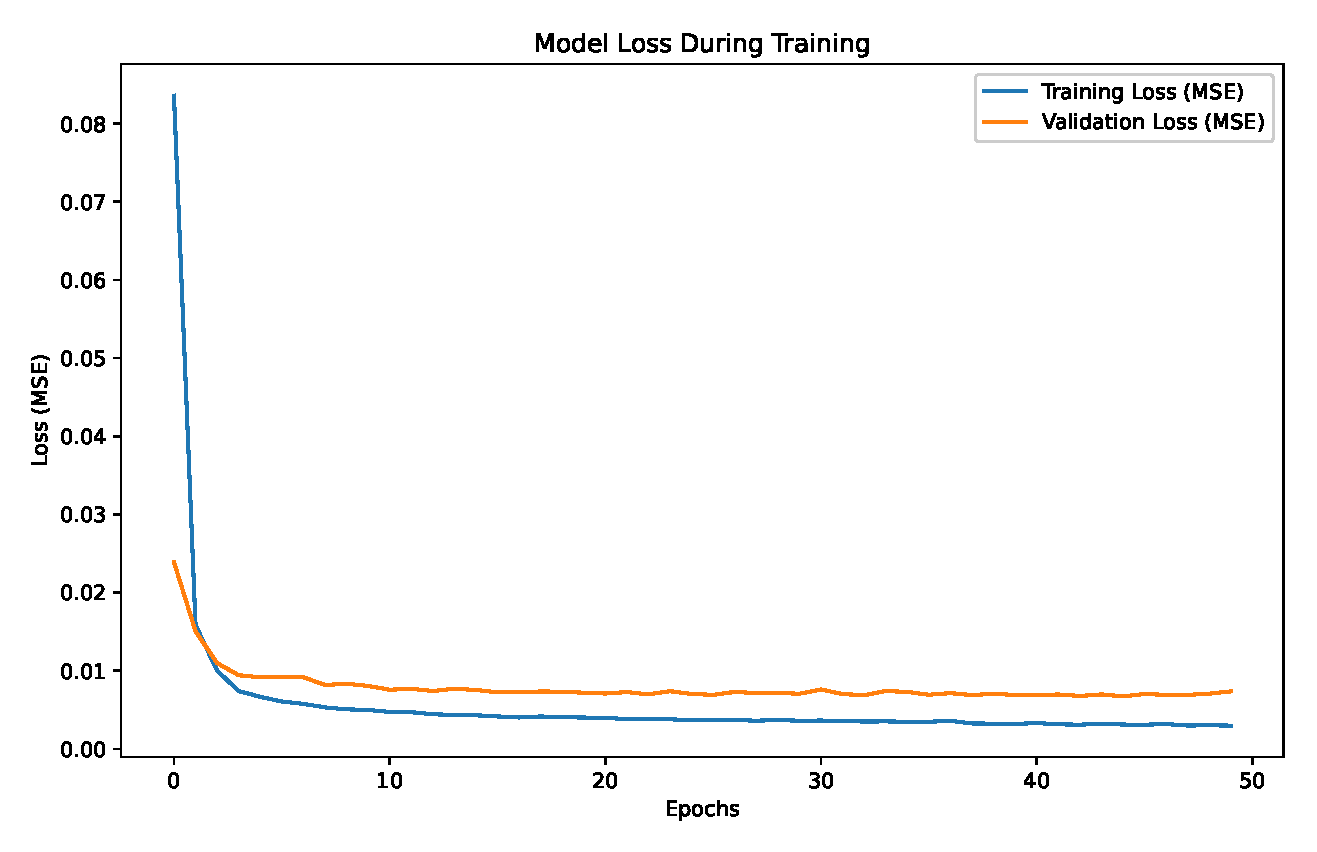
\includegraphics[width=0.45\textwidth]{images/loss_epochs.eps}
    \caption{Training and Validation Loss over Epochs}
    \label{fig:loss_epochs}
\end{figure}

To evaluate the model's performance further, the MSE loss was monitored for both the training and validation datasets across 50 epochs. As depicted in Fig~\ref{fig:loss_epochs}, the training loss steadily declined and plateaued around epoch 10. Similarly, the validation loss exhibited a comparable pattern, indicating that the model generalized well to unseen data with minimal signs of overfitting.

\subsection{Training and Validation Mean Absolute Error (MAE)}

\begin{figure}[htbp]
    \centering
    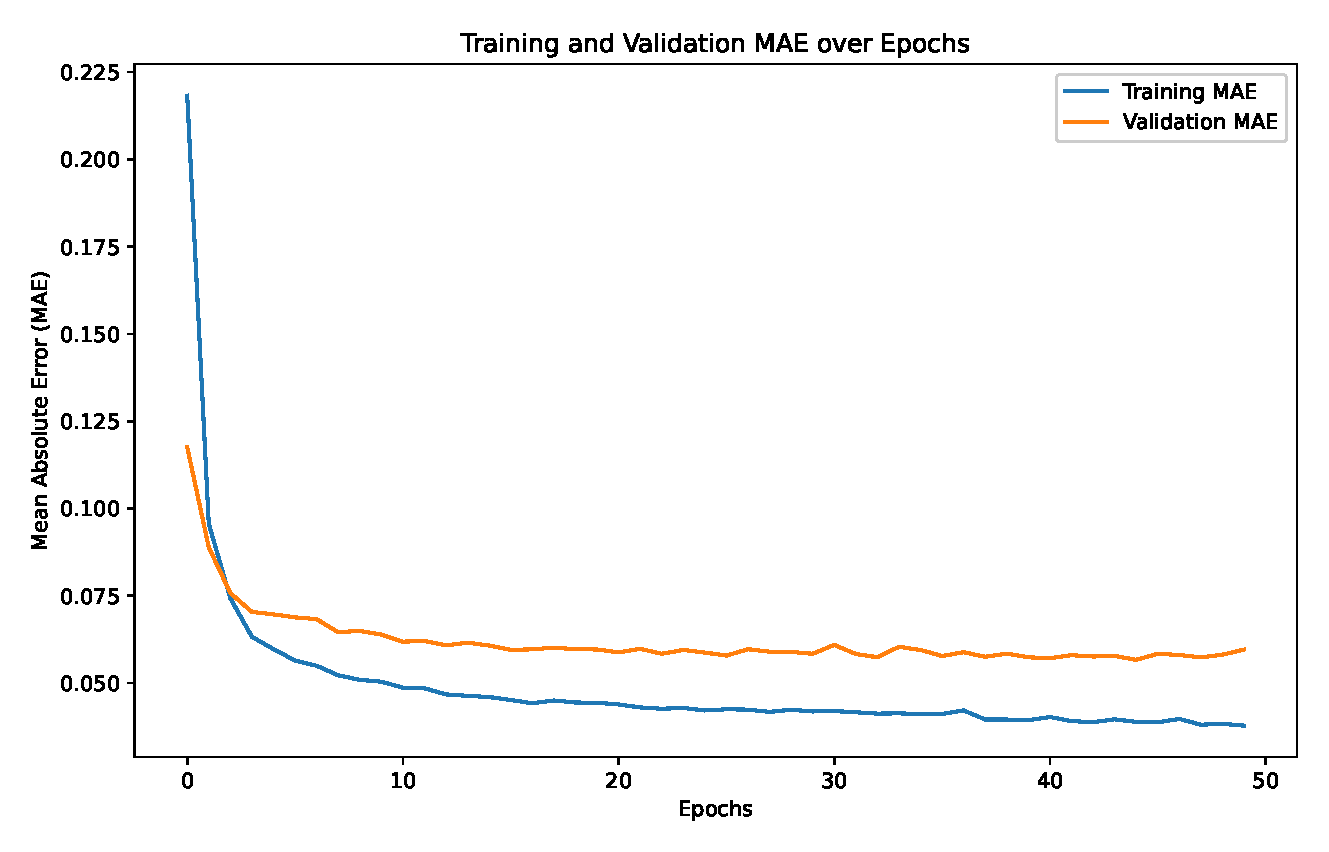
\includegraphics[width=0.45\textwidth]{images/mae_epochs.eps}
    \caption{Model MAE During Training and Validation}
    \label{fig:mae_epochs}
\end{figure}

Fig~\ref{fig:mae_epochs} illustrates the Mean Absolute Error (MAE) trends for both the training and validation datasets as the model progresses through the epochs. The graph demonstrates a steady reduction in training MAE, reflecting an improvement in the model's ability to minimize errors on the training data. The validation MAE also decreases initially, showcasing the model's capacity to generalize to unseen data, and stabilizes as training progresses. This trend indicates that the model avoids overfitting and achieves consistent performance across both datasets.


\subsection{Actual vs Predicted Traffic Flow}
\begin{figure}[htbp]
    \centering
    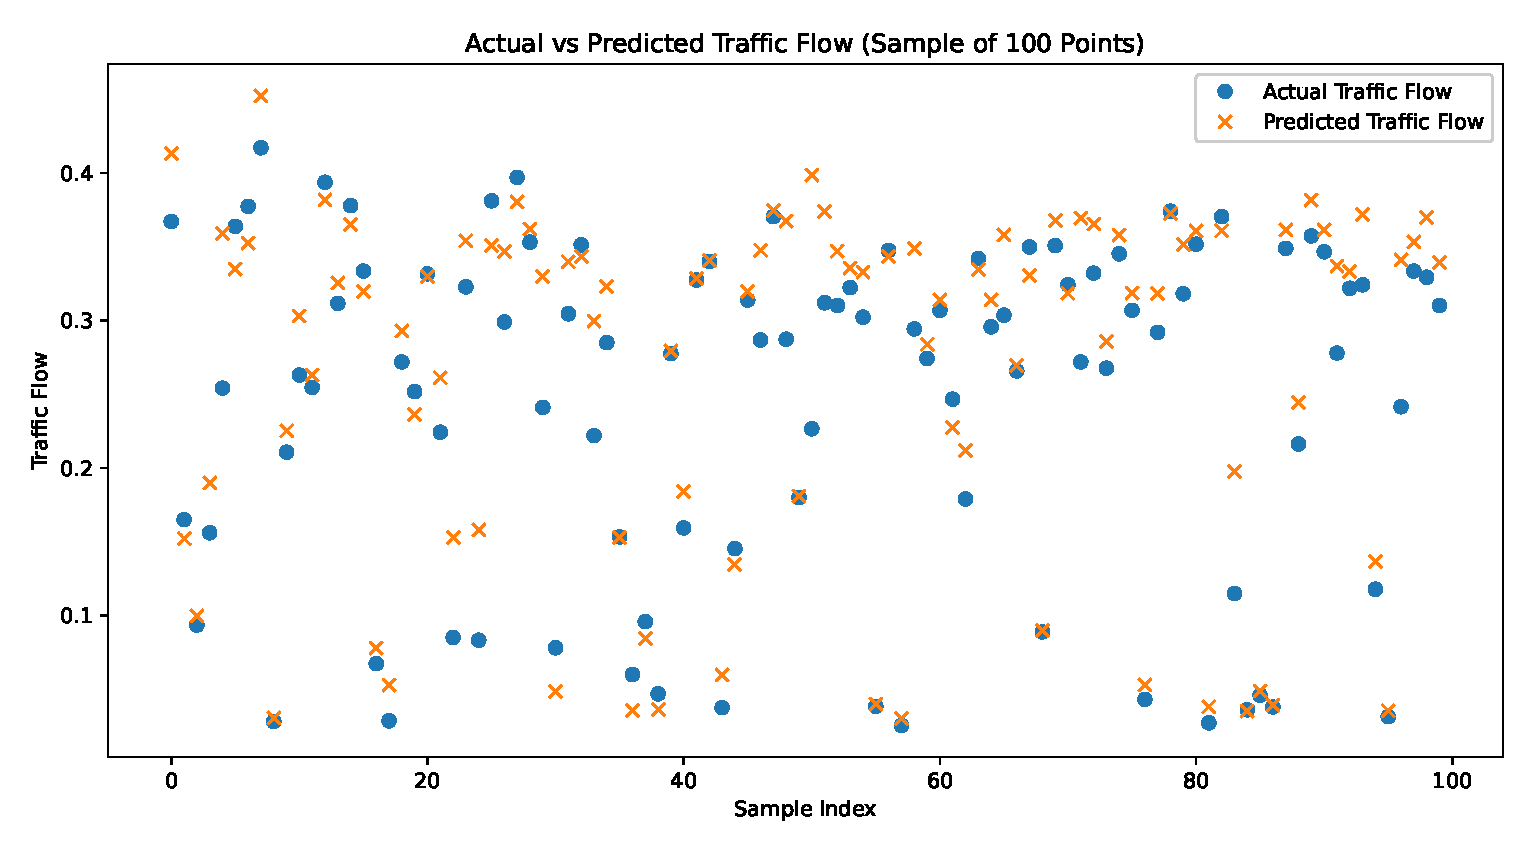
\includegraphics[width=0.45\textwidth]{images/actual_vs_predicted.eps}
    \caption{Actual vs Predicted Traffic Flow (Sample of 100 Points)}
    \label{fig:actual_vs_predicted}
\end{figure}

In Fig~\ref{fig:actual_vs_predicted}, the model’s predicted traffic flow closely aligns with the actual values over a sample of 100 data points. This strong alignment highlights the model’s ability to capture complex traffic flow patterns and accurately predict future traffic conditions.

\subsection{Error Distribution Across Sensor Locations}

To analyze the spatial distribution of errors, a heatmap of the mean squared error (MSE) across sensor locations was generated, as shown in Fig~\ref{fig:error_heatmap}. This visualization helps identify sensors with relatively higher prediction errors, providing insights into areas where the model encounters more complex traffic patterns.

\begin{figure}[htbp]
    \centering
    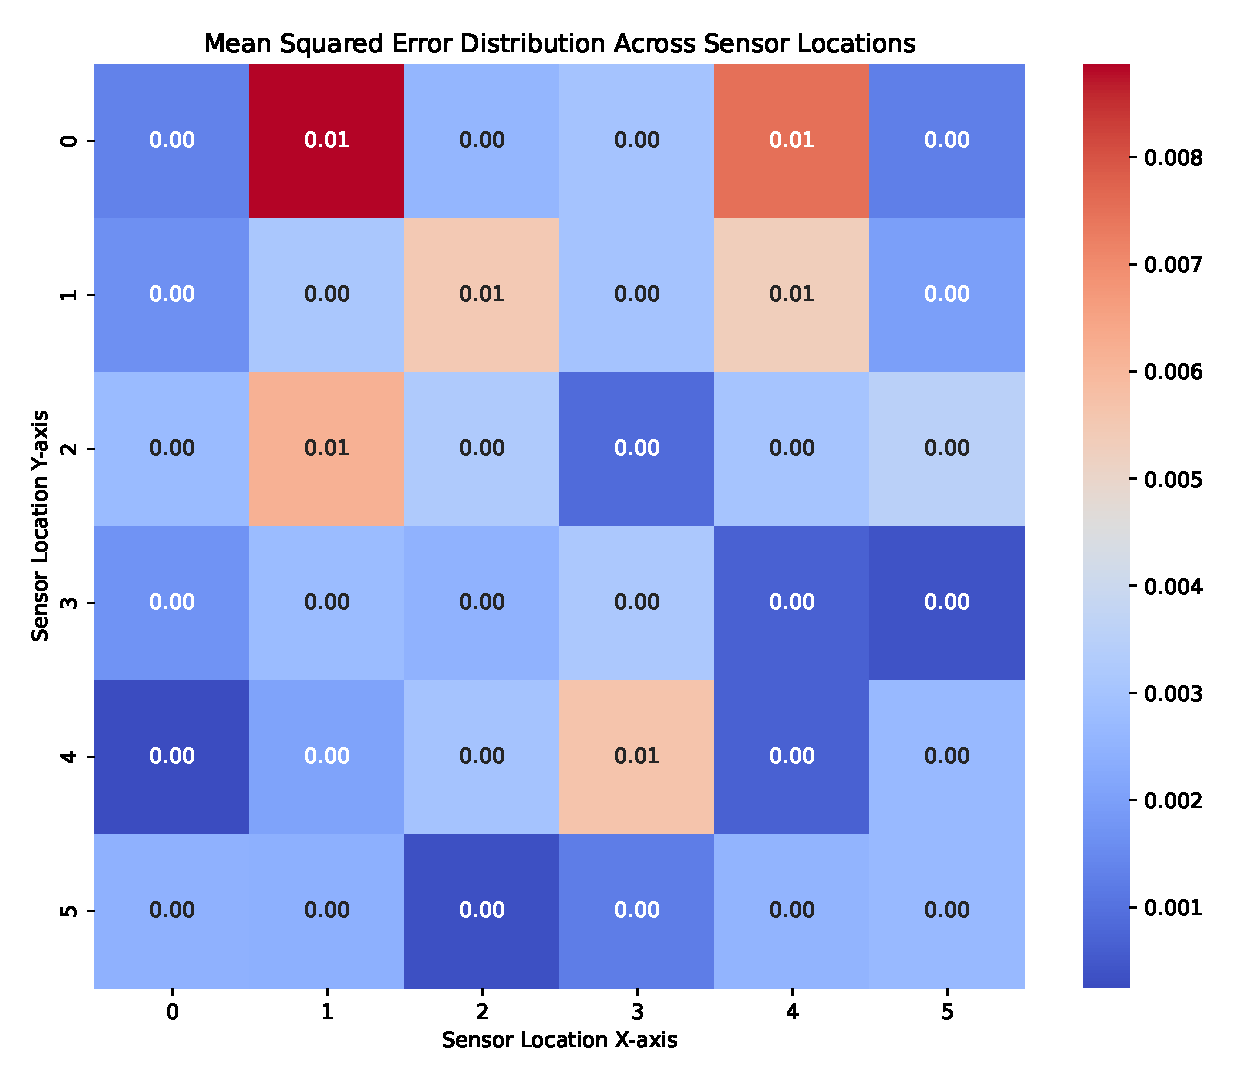
\includegraphics[width=0.4\textwidth]{images/error_heatmap.eps}
    \caption{Mean Squared Error Distribution Across Sensor Locations}
    \label{fig:error_heatmap}
\end{figure}

\subsection{Residual Error Histogram}

\begin{figure}[htbp]
    \centering
    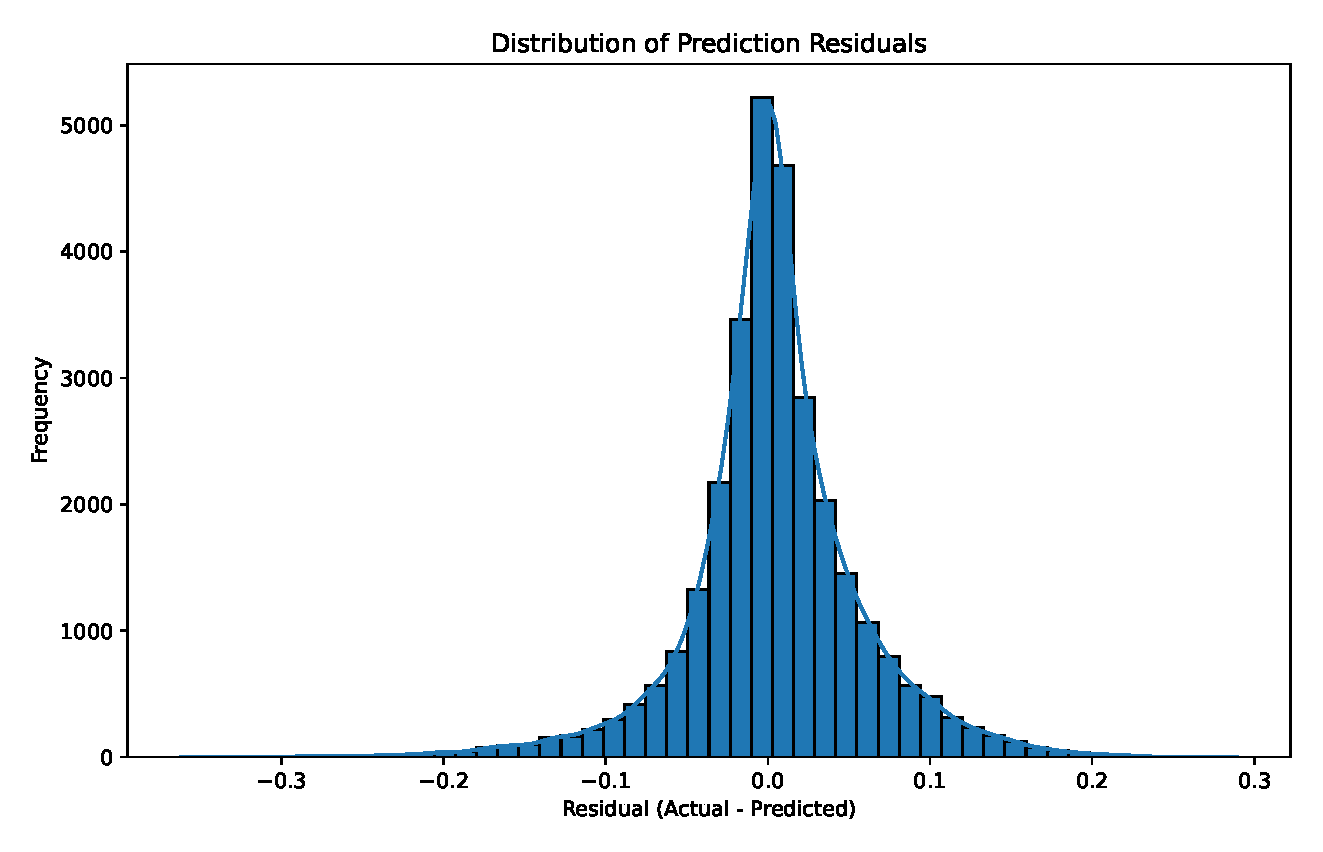
\includegraphics[width=0.4\textwidth]{images/residual_histogram.eps}
    \caption{Distribution of Prediction Residuals}
    \label{fig:residual_histogram}
\end{figure}

Fig~\ref{fig:residual_histogram} illustrates a histogram of the residuals, showing the differences between the actual and predicted traffic flow values. The distribution is centered and exhibits minimal skewness, suggesting that the model's predictions are unbiased and well-calibrated.

\section{Conclusion}

In this study, we developed a robust traffic flow prediction model using Long Short-Term Memory (LSTM) neural networks, utilizing spatiotemporal data from multiple sensors. The proposed model was shown to be effective in predicting traffic conditions with high accuracy and reliability, as demonstrated by key evaluation metrics such as an R² score of 0.8889, a mean squared error (MSE) of 0.0072, and a classification accuracy of 93.61\%. The results emphasize capturing complex patterns and dependencies in the traffic data that apply to making accurate and timely forecasts.

Our approach addresses the limitations of these traditional methods, such as ARIMA, and incorporates advanced deep learning techniques to improve prediction performances while maintaining scalability and adaptability. Including historical patterns of traffic, time dependencies, and contextual factors like weather provides a holistic understanding of the dynamics of traffic, allowing the model to be highly relevant to real-world scenarios.

This study's implications are far-reaching and very important in terms of traffic management systems, urban planning, and strategies for emergency response. The potential of our model to decrease congestion and improve road network efficiency will enhance the experiences of commuters and contribute to sustainable urban mobility. Future research could involve integrating real-time traffic data and expanding the model's scope to predict traffic disruptions caused by external factors such as accidents or construction.

In conclusion, this proposed LSTM-based traffic flow prediction system is a promising approach to the increasing challenges that urban traffic management faces today. It enables data-driven decision-making, paving the way toward smarter and more efficient transportation systems, ultimately benefiting the commuters, policymakers, and environment.






\section*{Acknowledgments}

The authors would like to acknowledge the financial support given by VIT Bhopal University, Bhopal-Indore Highway, Kothrikalan, Sehore Madhya Pradesh - 466114. Special thanks Dr.  Liang Zhao\cite{dataset} for the traffic dataset, without which this work would not have been possible. I would also like to extend my gratitude to my friends and family for their constant encouragement and motivation, making this endeavor achievable.








\begin{thebibliography}{99}
\bibitem{ppr25} Hanafy, Y.A., Mashaly, M.E., \& Abd El Ghany, M.A. (2021). An Efficient Hardware Design for a Low-Latency Traffic Flow Prediction System Using an Online Neural Network. Electronics.

\bibitem{ppr26} Sayed, S.A., Abdel-Hamid, Y., \& Hefny, H.A. (2023). Artificial intelligence-based traffic flow prediction: a comprehensive review. Journal of Electrical Systems and Information Technology, 10, 1-42.
\bibitem{dataset} Liang Zhao, Olga Gkountouna, and Dieter Pfoser. 2019. Spatial Auto-regressive Dependency Interpretable Learning Based on Spatial Topological Constraints. ACM Trans. Spatial Algorithms Syst. 5, 3, Article 19 (August 2019), 28 pages. DOI:\url{https://doi.org/10.1145/3339823}
\bibitem{same2018} M. Jiber, I. Lamouik, Y. Ali and M. A. Sabri, "Traffic flow prediction using neural network," 2018 International Conference on Intelligent Systems and Computer Vision (ISCV), Fez, Morocco, 2018, pp. 1-4, \url{https://doi.org/10.1109/ISACV.2018.8354066}

\bibitem{ppr1} Sayed, S.A., Abdel-Hamid, Y. \& Hefny, H.A. Artificial intelligence-based traffic flow prediction: a comprehensive review. Journal of Electrical Systems and Inf Technol 10, 13 (2023). \url{https://doi.org/10.1186/s43067-023-00081-6}


\bibitem{ppr2} Kashyap, A. A., Raviraj, S., Devarakonda, A., Nayak K, S. R., K V, S., Bhat, S. J., \& Galatioto, F. (2021). Traffic flow prediction models – A review of deep learning techniques. Cogent Engineering, 9(1). 
 \url{https://doi.org/10.1080/23311916.2021.2010510}

\bibitem{ppr3} Cini, N., Aydin, Z. A Deep Ensemble Approach for Long-Term Traffic Flow Prediction. Arab J Sci Eng 49, 12377–12392 (2024). 
 \url{https://doi.org/10.1007/s13369-023-08672-1}

\bibitem{ppr4} Nidhi, N., Lobiyal, D.K. Traffic flow prediction using support vector regression. Int. j. inf. tecnol. 14, 619–626 (2022). 
 \url{https://doi.org/10.1007/s41870-021-00852-2}

\bibitem{ppr5} Moumen, I., Abouchabaka, J., \& Rafalia, N. (2023). Adaptive traffic lights based on traffic flow prediction using machine learning models. International Journal of Electrical and Computer Engineering (IJECE), 13(5), 5813-5823. \url{http://doi.org/10.11591/ijece.v13i5.pp5813-5823}

\bibitem{ppr6} Deng, S., Jia, S., \& Chen, J. (2019). Exploring spatial–temporal relations via deep convolutional neural networks for traffic flow prediction with incomplete data. Applied Soft Computing, 78(open in a new window), 712–721. 
 \url{https://doi.org/10.1016/j.asoc.2018.09.040}

\bibitem{ppr7} Sun, S., Wu, H., \& Xiang, L. (2020, January). City-wide traffic flow forecasting using a deep convolutional neural network. Sensors (Switzerland), 20(open in a new window)(2(open in a new window) 421). \url{https://doi.org/10.3390/s200204}

\bibitem{ppr8} Osipov, V., Nikiforov, V., Zhukova, N., \& Miloserdov, D. (2020). Urban traffic flows forecasting by recurrent neural networks with spiral structures of layers. Neural Comput. Appl, 32(open in a new window), 14885–14897. \url{https://doi.org/10.1007/s00521-020-04843-5}

\bibitem{ppr9} Yang, B., Sun, S., Li, J., Lin, X., \& Tian, Y. (2019). Traffic flow prediction using LSTM with feature enhancement. Neurocomputing, 332(open in a new window), 320–327. \url{https://doi.org/10.1016/j.neucom.2018.12.016}

\bibitem{ppr10} Sayed, S.A., Abdel-Hamid, Y. \& Hefny, H.A. Artificial intelligence-based traffic flow prediction: a comprehensive review. Journal of Electrical Systems and Inf Technol 10, 13 (2023). \url{https://doi.org/10.1186/s43067-023-00081-6}

\bibitem{ppr11} Zhou Q, Chen N, Lin S. FASTNN: A Deep Learning Approach for Traffic Flow Prediction Considering Spatiotemporal Features. Sensors. 2022; 22(18):6921. 
 \url{https://doi.org/10.3390/s22186921}

\bibitem{ppr12} A. Khan, M. M. Fouda, D. -T. Do, A. Almaleh and A. U. Rahman, "Short-Term Traffic Prediction Using Deep Learning Long Short-Term Memory: Taxonomy, Applications, Challenges, and Future Trends," in IEEE Access, vol. 11, pp. 94371-94391, 2023 \url{https://doi.org/10.1109/ACCESS.2023.3309601}

\bibitem{ppr13} M. Fu, P. Wang, Z. Wang and Z. Li, "Deep Learning for Network Traffic Prediction: An Overview," 2023 IEEE Intl Conf on Dependable, Autonomic and Secure Computing, Intl Conf on Pervasive Intelligence and Computing, Intl Conf on Cloud and Big Data Computing, Intl Conf on Cyber Science and Technology Congress (DASC/PiCom/CBDCom/CyberSciTech), Abu Dhabi, United Arab Emirates, 2023, pp. 0665-0671 \url{https://doi.org/0.1109/DASC/PiCom/CBDCom/Cy59711.2023.10361459}

\bibitem{ppr14} H. Zheng, F. Lin, X. Feng and Y. Chen, "A Hybrid Deep Learning Model With Attention-Based Conv-LSTM Networks for Short-Term Traffic Flow Prediction," in IEEE Transactions on Intelligent Transportation Systems, vol. 22, no. 11, pp. 6910-6920, Nov. 2021 \url{https://doi.org/10.1109/TITS.2020.2997352}

\bibitem{ppr15} Sroczyński, A., Czyżewski, A. Road traffic can be predicted by machine learning equally effectively as by complex microscopic model. Sci Rep 13, 14523 (2023). \url{https://doi.org/10.1038/s41598-023-41902-y}

\bibitem{ppr16} X. Zhang, K. Huang, C. Liu and X. Xu, "Urban Short - Term Traffic Flow Prediction Algorithm Based on CNN-LSTM Model," 2023 3rd International Conference on Consumer Electronics and Computer Engineering (ICCECE), Guangzhou, China, 2023, pp. 214-217 \url{https://doi.org/10.1109/ICCECE58074.2023.10135384}

\bibitem{ppr17} Manuel Méndez, Mercedes G. Merayo, Manuel Núñez,
Long-term traffic flow forecasting using a hybrid CNN-BiLSTM model,
Engineering Applications of Artificial Intelligence,Volume 121,2023,106041,ISSN 0952-1976 \url{https://doi.org/10.1016/j.engappai.2023.106041}

\bibitem{ppr18} Wang, S., Shao, C., Zhang, J. et al. Traffic flow prediction using bi-directional gated recurrent unit method. Urban Info 1, 16 (2022). \url{https://doi.org/10.1007/s44212-022-00015-z}

\bibitem{ppr19} Wen, W., Xu, D., \& Xia, Y. (2023). A novel traffic optimization method using GRU based deep neural network for the IoV system. PeerJ. Computer science, 9, e1411. \url{https://doi.org/10.7717/peerj-cs.1411}

\bibitem{ppr20} W. Zhang, X. Li, A. Li, X. Huang, T. Wang and H. Gao, "SGRU: A High-Performance Structured Gated Recurrent Unit for Traffic Flow Prediction," 2023 IEEE 29th International Conference on Parallel and Distributed Systems (ICPADS), Ocean Flower Island, China, 2023, pp. 467-473 \url{https://doi.org/10.1109/ICPADS60453.2023.00076}

\bibitem{ppr21} Zhao, Y., Han, X., \& Xu, X. (2022). Traffic flow prediction model based on the combination of improved gated recurrent unit and graph convolutional network. Frontiers in bioengineering and biotechnology, 10, 804454.

\bibitem{ppr22} Jang, H.-C.; Chen, C.-A. Urban Traffic Flow Prediction Using LSTM and GRU. Eng. Proc. 2023, 55, 86. \url{https://doi.org/10.3390/engproc2023055086}

\bibitem{ppr23} Yu, L., Zhao, J., Gao, Y., \& Lin, W. (2019, June). Short-term traffic flow prediction based on deep learning network. In 2019 international conference on robots \& intelligent system (ICRIS) (pp. 466-469). IEEE.

\bibitem{ppr24} Zhang, Q., et al. "Short-term multi-step-ahead sector-based traffic flow prediction based on the attention-enhanced graph convolutional LSTM network (AGC-LSTM)." Neural Computing and Applications, 2024, \url{https://doi.org/10.1007/s00521-024-09827-3}



\end{thebibliography}



\end{document}
